\documentclass{article}

\usepackage{amsmath,amssymb}
\usepackage{graphicx}
\usepackage{array}
\usepackage[margin=1in]{geometry}
\usepackage{dsfont}

% ===== This makes my \affil cmnd work.
\usepackage[affil-it]{authblk}


% ===== This makes my environments work switching llncs to article.
\newtheorem{theorem}{Theorem}[section]
\newtheorem{lemma}[theorem]{Lemma}
\newtheorem{proposition}[theorem]{Proposition}
\newtheorem{corollary}[theorem]{Corollary}

\newenvironment{proof}[1][Proof]{\begin{trivlist}
\item[\hskip \labelsep {\bfseries #1}]}{\end{trivlist}}
\newenvironment{definition}[1][Definition]{\begin{trivlist}
\item[\hskip \labelsep {\bfseries #1}]}{\end{trivlist}}
\newenvironment{example}[1][Example]{\begin{trivlist}
\item[\hskip \labelsep {\bfseries #1}]}{\end{trivlist}}
\newenvironment{remark}[1][Remark]{\begin{trivlist}
\item[\hskip \labelsep {\bfseries #1}]}{\end{trivlist}}

\newcommand{\qed}{\nobreak \ifvmode \relax \else
      \ifdim\lastskip<1.5em \hskip-\lastskip
      \hskip1.5em plus0em minus0.5em \fi \nobreak
      \vrule height0.75em width0.5em depth0.25em\fi}

% ===== For \algorithm. Is this a decent idea?
\usepackage[lined,boxed,ruled,vlined]{algorithm2e}

% ===== For \mathscr
\usepackage{mathrsfs}
\DeclareSymbolFontAlphabet{\mathrsfs}{rsfs}
\usepackage[mathscr]{eucal}


% ===== For \boldsymbol
\usepackage{amsbsy}

% ===== For \bm (bold math)
\usepackage{bm}

\usepackage{fixltx2e}
\MakeRobust{\overrightarrow}

% ===== For code snippets
\usepackage{courier}

% ==== Misha and Ning's Notation file =====
%% ----------------------------------------------------------------------
%% Definitions, Macros, Etc.
%% ----------------------------------------------------------------------

%% Hyper-linked References
\newcommand{\Sec}[1]{\hyperref[sec:#1]{\S\ref*{sec:#1}}} %section
\newcommand{\Eqn}[1]{\hyperref[eq:#1]{(\ref*{eq:#1})}} %equation
\newcommand{\Fig}[1]{\hyperref[fig:#1]{Figure~\ref*{fig:#1}}} %figure
\newcommand{\Tab}[1]{\hyperref[tab:#1]{Table~\ref*{tab:#1}}} %table
\newcommand{\Thm}[1]{\hyperref[thm:#1]{Theorem~\ref*{thm:#1}}} %theorem
\newcommand{\Lem}[1]{\hyperref[lem:#1]{Lemma~\ref*{lem:#1}}} %lemma
\newcommand{\Prop}[1]{\hyperref[prop:#1]{Property~\ref*{prop:#1}}} %property
\newcommand{\Cor}[1]{\hyperref[cor:#1]{Corollary~\ref*{cor:#1}}} %corollary
\newcommand{\Def}[1]{\hyperref[def:#1]{Definition~\ref*{def:#1}}} %definition
\newcommand{\Alg}[1]{\hyperref[alg:#1]{Algorithm~\ref*{alg:#1}}} %algorithm
\newcommand{\Ex}[1]{\hyperref[ex:#1]{Example~\ref*{ex:#1}}} %example

% Theorem-like constructs
%\newtheorem{example}[theorem]{Example}

% Blackboard fonts 
\newcommand{\Real}{\mathbb{R}}
\newcommand{\Cplx}{\mathbb{C}}
%% Transposes
\newcommand{\Tra}{^{\rm T}} % Transpose
\newcommand{\Cct}{^\dagger} % Complex conjugate transpose

%% Permutation index
\newcommand{\bfpp}{{\bf p}_n}

%% Matrix & Tensor Operations
\newcommand{\Circ}[1]{{\rm circ}\left( #1 \right)}
\newcommand{\Fold}[1]{{\rm fold}\left( #1 \right)}
\newcommand{\Unfold}[1]{{\rm unfold}\left( #1 \right)}
\newcommand{\Twist}[1]{{\rm twist}(\M{#1})}
\newcommand{\Squeeze}[1]{{\rm squeeze}(#1)}
\newcommand{\squeeze}{{\rm squeeze}}
\newcommand{\Mout}{\diamondsuit}
\newcommand{\circu}{ {\rm circ}}
\newcommand{\bcirc}{ {\rm circ}}
\newcommand{\vvec}{ {\rm vec}}

\newcommand{\mc}[1]{\mathcal{#1}}
\newcommand{\mb}[1]{\mathbb{#1}}
\newcommand{\mcr}[1]{\mathrsfs{#1}}

%% Element of complicated object that is surrounded by parens
\newcommand{\PE}[2]{\left( #1 \right)_{#2}}

%% Vector notation
\newcommand{\V}[1]{{\bm{\mathbf{\MakeLowercase{#1}}}}} % vector
\newcommand{\VE}[2]{\MakeLowercase{#1}_{#2}} % vector element

%% Matrix notation
\newcommand{\M}[1]{{\bm{\mathbf{\MakeUppercase{#1}}}}} % matrix
\newcommand{\Mhat}[1]{{\bm{\hat \mathbf{\MakeUppercase{#1}}}}} % matrix
\newcommand{\Mbar}[1]{{\bm{\bar \mathbf{\MakeUppercase{#1}}}}} % matrix
\newcommand{\ME}[2]{\MakeLowercase{#1}_{#2}} % matrix element
\newcommand{\MC}[2]{\V{#1}_{#2}}

%% Tensor notation
\newcommand{\T}[1]{\boldsymbol{\mathscr{\MakeUppercase{#1}}}} %tensor
\newcommand{\TLS}[2]{\M{#1}_{[#2]}} % lateral slice
\newcommand{\TFS}[2]{\M{#1}_{#2}} % frontal slice
\newcommand{\TT}[2]{\V{#1}_{#2}} % tube
\newcommand{\TE}[2]{\MakeLowercase{#1}_{#2}} % tensor element


%% Shortcuts
\newcommand{\TA}{\T{A}}
\newcommand{\TB}{\T{B}}
\newcommand{\TS}{\T{S}}
\newcommand{\TC}{\T{C}}
\newcommand{\TU}{\T{U}}
\newcommand{\TV}{\T{V}}
\newcommand{\TG}{\T{G}}

\newcommand{\Vu}{\V{u}}
\newcommand{\Vv}{\V{v}}
\newcommand{\Vq}{\V{q}}
\newcommand{\Vr}{\V{r}}
\newcommand{\Vp}{\V{p}}
\newcommand{\Vd}{\V{d}}
\newcommand{\Vz}{\V{z}}
\newcommand{\Vb}{\V{b}}
\newcommand{\Vg}{\V{g}}
\newcommand{\Vh}{\V{h}}
\newcommand{\MH}{\M{H}}
\newcommand{\MG}{\M{G}}
\newcommand{\MA}{\M{A}}
\newcommand{\MX}{\M{X}}
\newcommand{\MZ}{\M{Z}}
\newcommand{\MW}{\M{W}}
%\newcommand{\TD}{\T{D}}

\newcommand{\SaS}{{\mathcal S}}

\newcommand{\MGC}{\tilde{\MG}}

\newcommand{\Matlab}{{\sc Matlab}\xspace}
\newcommand{\matlab}{{\sc Matlab}\xspace}
\newcommand{\qtext}[1]{\quad\text{#1}\quad}

\newcommand{\matvec}{{\tt Vec}}
\newcommand{\fld}{{\tt Fold}}

\def \bK{\mathbf{K}}
\def \bF{\mathbf{F}}
\def \bD{\mathbf{D}}
\def \bB{\mathbf{B}}
\def \bA{\mathbf{A}}
\newcommand{\bDelta}{\boldsymbol{\Delta}}

%\newcommand{\bea}{\left[ \begin{array}}
%\newcommand{\eea}{ \end{array} \right]} 

\newcommand{\bftheta}{ {\boldsymbol \theta}}
\newcommand{\bfrho}{ {\boldsymbol \rho}}
\newcommand{\bfeta}{ {\boldsymbol \eta}}
\newcommand{\fft}{ \mbox{\tt fft} }
\newcommand{\ifft}{ \mbox{\tt ifft} }
\newcommand{\blkd}{\mbox{\tt blkdiag}}
\newcommand{\rshpT}{\mbox{\tt reshapeT}}
\newcommand{\F}[1]{\mathcal{F}\{#1\}}
\newcommand{\Fi}[1]{\mathcal{F}^{-1}\{#1\}}
\newcommand{\indep}{\perp\!\!\!\perp}

\usepackage{mathtools}
\DeclarePairedDelimiter{\ceil}{\lceil}{\rceil}
\DeclarePairedDelimiter{\floor}{\lfloor}{\rfloor}
\newcommand{\Var}{\text{Var}}
\newcommand{\E}{\text{E}}
\newcommand{\Cov}{\text{Cov}}



%%%% Dr. K's colored comments. 
\usepackage{color} 
\definecolor{blue}{rgb}{0,0,1}
\definecolor{red}{rgb}{1,0,0}
\definecolor{purple}{rgb}{1,0,1}
\definecolor{gray}{rgb}{0.7,0.7,0.7}
\newcommand\MEK[1]{\textcolor{red}{MEK: #1}}
\newcommand\EMK[1]{\textcolor{purple}{EMK: #1}}
\newcommand\SA[1]{\textcolor{blue}{SA: #1}}
\newcommand\red[1]{\textcolor{red}{#1}}\newcommand\gray[1]{\textcolor{gray}{#1}}
\begin{document}



Eric Kernfeld

Report on Darren Wilkinson's ``Parameter inference for stochastic kinetic models of bacterial gene regulation,'' also referred to as ``the paper'' or ``W09.'' It is a chapter in the proceedings of the ninth Valencia meeting on Bayesian statistics \cite{Bernardo2012}. 

\begin{abstract}
In this paper, Wilkinson attempts to infer reaction rates for biochemical networks in a setting with discrete observations, missing data, and measurement error. He uses vague priors and likelihood-free MCMC methods within a Bayesian model. He runs four main simulations. The first three iterate through successively more difficult and realistic measurement models, and they show the approach can accurately infer three key reaction rates with a useful precision. The fourth studies a naive model, showing it leads to overconfident, incorrect inferences. 

I review some alternative methods in detail and discuss the relative merits of W09's approach. I implement the method in Julia and attempt to reproduce the experiments \EMK{more on this later!}. I assess the method using additional experiments designed to study mixing time, scaling with system size, and prior sensitivity \EMK{more on this later!}. 
\end{abstract}


\section{Introduction: Parameter Inference for Biological Models}

Modern biology has progressed to the point of creating {\it in silico} models of entire cells. The potential benefit is enormous, because unlike real cells, which must be observed via microscopy or high-throughput methods, a simulated cell can regularly dump its entire internal state to a file. The obvious drawback is that simulations do not necessarily correspond to reality either in terms of their mechanisms or in terms of their results. One key limiting factor is this: even though the structure of biochemical networks is often well known, precise information about how quickly interactions play out has not kept pace. If Protein A promotes transcription of Gene B, and we let them mix for five minutes, we still need to know whether to expect 10, 100 or 1000 new copies of B's messenger RNA at the end. Wilkinson's paper (W09) confronts a subproblem in this domain.

Chemical reactions are often modeled using ordinary differential equations (ODE's), but Wilkinson's exact subproblem has an extra complication that rules ODE's out: natural stochasticity. W09's model organism, the bacterium {\it Bacillus subtilis}, varies its behavior so that even if two bacteria begin in similar initial conditions, one may become mobile and the other may not. Here is one explanation, which the underlying physics support and which  Wilkinson's paper subscribes to. Interactions among molecules are themselves random, driven by Brownian motion. If there are only tens or hundreds of molecules, the randomness persists in the system dynamics rather than canceling out. Some natural systems even amplify it in order to produce usefully random behavior \cite{reinker2006parameter}. Wilkinson expresses this in terms of a particular stochastic model, and the main contribution of his paper is a method for inference assuming that model.
 
%In some cases, organisms have mechanisms to reduce this randomness, but in others, as readers fond of rock-paper-scissors might imagine, the random behavior is useful.

\subsection{Poisson process modeling of chemical systems}

For a well-stirred chemical system that maintains thermal equilibrium, Gillespie  \cite{gillespie1992rigorous} derived a model from first principles. The ultimate result is a collection of competing Poisson processes, one for each chemical reaction to be modeled. Suppose there are $X_{i}(t)$ molecules of type $i$ at time $t$, $i\in \{1 ... u\}$. These molecules interact via a set of reactions $\mathcal{R}_{j}$, $j\in \{1 ... v\}$, with $\mathcal{R}_{j}$ consuming $p_{ij}$ particles of type $i$ and producing $q_{ij}$ particles of type $i$. Let $R_{j}(t)$ denote the number of reactions of type $j$ that happened in $[0,t]$. I'll refer to all these variables collectively using the time-varying vectors $X(t)$ and $R(t)$ along with static matrices $P$ and $Q$. Defining the matrix $S$ to be $Q-P$, the equation $X(t) - X(0) = SR(t)$ shows how the reactions affect the molecule counts. Since the particle counts are integers, the system is not constantly in flux: there will be windows, perhaps short ones, where no reactions occur. The exact form of the model is this: over a reaction-free window, $R_{j}(t)$ is a Poisson process with intensity $c_{j}\int_0^t \prod_{i=1}^u {{X_i(t)}\choose{p_{ij}}}$. %Define $h_{i}(c_{i}, X(t)) \equiv c_{i}\int_0^t \prod_{j=1}^u {{X_j(t)}\choose{p_{ij}}}$. 
The $c_{i}$'s are sometimes unknown, and they are the quantities needed for biological models.

\subsection{Inference with complete data and simulation}
Given that every reaction is observed without error, inference is still needed because the system is stochastic. To rapidly understand the likelihood, think of how to simulate the system.

As with any homogeneous Poisson process, draw an exponential random variable with rate equal to the intensity of the process; that gives the correctly distributed waiting time until the next event. For a collection of independent Poisson processes, use the sum of their intensities as the rate. Choose the type of reaction from a categorical distribution with cell probabilities equal to the normalized intensities. This scheme applies to this setting because even though the process is not homogeneous, it is temporarily homogenous in between reactions. The rates can be recomputed after each new reaction. Popularized by  \cite{gillespie1977}, this is known as the Gillespie algorithm. Pseudocode appears in Algorithm \ref{alg:gillespie}.


\begin{algorithm}[h]
\caption{The Gillespie algorithm \label{alg:gillespie}}
Given:\\
\Indp
A simulation duration $T$\\
$X(0)$, the initial particle counts\\
$S$, a ``stoichiometry matrix'' whose $i,j$ entry says how many molecules of type $i$ appear or vanish in a reaction of type $j$ (net change)\\
$P$, a matrix whose $i,j$ entry says how many molecules of type $i$ enter a rxn of type $j$ (not a net change)\\
$c$, a vector of reaction rates\\
-\\
\Indm
Do this:\\
\Indp
Initialize $X$ to $X(0)$ and $t$ to 0.\\
While true:\\
\Indp
Calculate $\alpha_j = c_j\prod_i {X_i\choose P_{ij}}$\\
Increment $t$ by Exponential($\sum_j \alpha_j$) ($\sum_j \alpha_j$ is the rate parameter)\\
If $t > T$, quit and return $X$.\\
Otherwise, choose an integer $j$ with probability $\frac{\alpha_j}{\sum_j \alpha_j}$.\\
Increment $X$ by adding column $j$ of $S$.\\
\end{algorithm}


Returning to the likelihood, suppose $\nu$ is a vector so that the $i$th reaction has type $\nu_i$ and $t$ is a vector so that the $i$th reaction happens at time $t_i$. The likelihood has a term corresponding to the exponential with the sum of the Poisson intensities. Conditioned on the wait times, the next term consists of the categorical probability given to the actual reaction type observed. That happens for every observed reaction. The normalizing constants of the factors cancel, and the final formula is $$L(c|\nu, t) = \prod_{i=1}^n c_{\nu_{i}} \prod_{j=1}^u {{X_{j}(t_{i-1})}\choose{p_{{\nu_{i}}j}}}\exp\left(-c_{\nu_{i}}\sum_{i=1}^{n} (t_{i}-t_{i-1}) {{X_j(t_{i})}\choose{p_{{\nu_{i}}j}}}\right).$$

In terms of maximum likelihood inference, this function and its derivatives can be evaluated. In terms of Bayesian inference, it has a conjugate prior (independent Gamma distributions). Computational scale is not an issue: Wilkinson's examples have only 13 molecule types and 18 reactions. The problem arises because of discretely observed data.

\subsection{Approaching inference without complete data}
\label{sec:intro_em}
In Wilkinson's data, not every reaction is observed. Rather, measurements of molecule counts are taken every five minutes. Many possible sequences of reactions could have resulted in the same observations (infinitely many, counting production-decay or binding-unbinding loops). For each sequence, uncountably many variations exist: consider stretching or shrinking the wait times. Let $\nu$ range over the set of eligible reaction sequences, meaning it matches the observed data. Let $\Omega_{\nu}$ be the set of possible times for reactions in $\nu$. The likelihood becomes 
\begin{equation}\label{eqn_nasty_lik}
L(c|X(0), X(t_1), ... X(T)) =\sum_{\nu}\int_{t\in \Omega_{\nu}} \prod_{i=1}^n c_{\nu_{i}} \prod_{j=1}^u {{X_{j}(t_{i-1})}\choose{p_{{\nu_{i}}j}}}\exp\left(-c_{\nu_{i}}\sum_{i=1}^{n} (t_{i}-t_{i-1}) {{X_j(t_{i})}\choose{p_{{\nu_{i}}j}}}\right).
\end{equation}
 The domain of integration $\Omega_{\nu}$ has dimension $n$, and $n$ changes depending on $\nu$. Most reaction sequences are ineligible, if we define ``most'' via a the measure induced by simulation. In other words, most forward simulations, even with correct initial conditions, will not match the data. 

To my knowledge, this likelihood has not been evaluated. Instead, expectation-maximization is a common recourse: alternate between updating parameters and calculating expected latent reaction times/types. Since calculating expected latent reaction times and types is not necessarily possible, as it would be in the case of a time-homogenous process, Horv\'ath and Manini \cite{horvath2008parameter} instead draw samples using the Gillespie method. This produces mostly trajectories at odds with the observations, so after a few simulations, they discard all but the trajectory closest to fitting the data, and then they tweak this trajectory by altering some reactions. This makes their method inexact, though they argue the distortion of the likelihood is minimal unless molecule counts are close to zero. Daigle et al. \cite{daigle2012accelerated} take a very similar tactic, also using EM with a sampling-based E-step done by rejecting incorrect trajectories. To reduce wasted simulation time, Daigle et al. use a tool they call multi-level splitting, and it bears an eerie resemblence to the MCMC method that Wilkinson contributes.  Another EM-based method contributed by Bayer et al. \cite{bayer2015stoch_em} confronts the same problem of how to obtain trajectories consistent with data. Their scheme is to simulate forward from one observed time-point and backwards from the next, hoping the two samples meet in the middle. A common theme in this domain is that careful initialization helps reduce the fraction of useless samples. This idea, too, will be mirrored in the Bayesian literature on the topic.

In Wilkinson's work, some molecule counts are zero or close to zero, which renders the approximation in \cite{horvath2008parameter} dubious. Though missing data has not yet been mentioned, at time $t_i$, Wilkinson observes only one molecule out of a system with 13, or in other words one coordinate of the 13-dimensional vector $X(t_i)$. This disqualifies \cite{bayer2015stoch_em} by Bayer et al.'s own admission. The method by Daigle et al., \cite{daigle2012accelerated}, can accomodate partial observations, so it remains competitive, and furthermore it claims to beat a different paper co-authored by Wilkinson \cite{Boys2008}. However, \cite{daigle2012accelerated} was not published when Wilkinson came out with the method reproduced here.

%Even if competitive EM-based methods had been available in 2009, 
Wilkinson's papers tend to use Bayesian methods, and they tend to use MCMC for inference. A 2003 paper by Marjoram et al. \cite{Marjoram23122003} opened the way for Metropolis-Hastings samplers that do not require likelihood evaluations. Wilkinson introduces one of these, claims it will not work, and makes, as his paper's main contribution, an adaptation of likelihood-free MCMC (LF-MCMC) for hidden discrete or continuous-time Markov models.

\subsection{Methods similar to Wilkinson's}
\label{MC_backgr}
Wilkinson's adaptation of LF-MCMC is subtle and strange. Because it contains ingredients of several Monte Carlo schemes, the discussion leading up to Wilkinson's algorithm will briefly detour through sequential Monte Carlo and LF-MCMC. Readers familiar with these schemes may wish to skip to the pseudocode in Algorithm \ref{pMCMC} and the attending description. 

On its own, LF-MCMC is just a form of Metropolis-Hastings. To produce samples from a {\it target distribution} $\pi$ over a hidden state $x$ and parameters $\theta$, recall that Metropolis-Hastings says to propose a new sample $x^*, \theta^*$ with distribution $q(x^*, \theta^*|x, \theta)$, then accept the proposal with probability $\min \{1, A\}$ if $A=\frac{q(x, \theta|x^*, \theta^*)}{q(x^*, \theta^*|x, \theta)} \times \frac{\pi(x^*, \theta^*)}{\pi(x, \theta)}$. It will help to keep in mind this ``recipe'' for Metropolis-Hastings, but to motivate and describe LF-MCMC, we move back to the stochastic chemical model.

Suppose we have a set of observations at times $t_i$, $i \in 1...I$, and for each $i$ we label the observations $D_{t_i}$. These might be real-valued scalars. The observations depend on the current hidden state, which is the vector of counts for each molecule type. They may also depend on $\theta$, which aggregates parameters of the measurement error model along with any unknown reaction rates. At time $t_i$, Wilkinson observes only one coordinate of the 13-dimensional vector $X(t_i)$, and it is a noisy observation. On the bright side, the revealed coordinate is fixed and known, and $P(D_{t_{i}}|x_{t_i}, \theta)$ is assumed to be tractable. So is the prior $P(\theta)$. Since the target distribution for the MCMC is the posterior $P(x, \theta|D)$, the term $\frac{P(x^*, \theta^*|D)}{P(x, \theta|D)}$ can be rewritten $\frac{P(D|x^*, \theta^*)P(x^*|\theta^*)P(\theta^*)}{P(D|x, \theta)P(x| \theta)P(\theta)}$. The only intractable calculation is $P(x^*|\theta^*)$, a special case of Equation \ref{eqn_nasty_lik}. To avoid it, the LF-MCMC comes in.

Marjoram et al. dodge this type of problem not by approximation, but by making the intractable term appear in a second location. In Metropolis-Hastings, each iteration needs the quantity $A=\frac{q(x, \theta|x^*, \theta^*)}{q(x^*, \theta^*|x, \theta)} \times \frac{\pi(x^*, \theta^*)}{\pi(x, \theta)}$. Noticing that the asterisks appear in the numerator for $q$ and the denominator for $\pi$, the inspiration is to build $P(x| \theta)$ into the {\it proposal}. By proposing only $\theta$, then simulating $x$ from the correctly-formed model (here, via the Gillespie algorithm), the entire thing becomes $A=\frac{q(\theta|\theta^*)}{q(\theta^*|\theta)} \frac{P(x|\theta)}{P(x^*|\theta^*)} \times \frac{P(D|x^*, \theta^*)P(x^*|\theta^*)P(\theta^*)}{P(D|x, \theta)P(x| \theta)P(\theta)}$. The intractable terms cancel.

Wilkinson points out that this scheme suffers from the same problem that besets the sampling-based EM: most forward simulations are incongruent with the data. Once the chain gets to taste a single well-placed sample sequence of reactions, it is unlikely to explore parameters and initial conditions other than what produced the winning simulation. The rejection rate is high, and the mixing time is bad. Wilkinson reasonably claims that this problem gets worse with less measurement error or with higher-dimensional observations, and that Marjoram et al.'s method will not work ``out of the box.'' He offers no theory, citations, or experiments to support this claim, except for a clause containing the phrase ``in practice,'' which implies experiments not reported in this paper. Wilkinson's work centers around building a sampler with tolerable rejection rates. 

The idea is similar to sequential Monte Carlo (SMC), which uses a sequence of distributions rather than moving directly from proposal to posterior. Most SMC methods resemble importance sampling: propose a collection of independent, identically distributed samples from the wrong distribution. To render the result unbiased, calculate functionals only after appropriately up- or down-weighting each of the samples. 

As is done in this branch of MCMC research, I will begin to refer to each individual sample as a particle. SMC solves a problem where most particle weights become small, and just a few particles contribute most of the information. The SMC solution is to introduce several intermediate stages of resampling in which successful particles can multiply and low-weight particles can vanish. Some strategies use perturbations so that the duplicate particles disperse during resampling. If the weights at intermediate stages come from distributions that progress gradually from proposal to target, the effect is a particle cloud slowly migrating into the correct formation, where simple importance sampling would produce a particle cloud whose body all but vanishes and whose wispy edges determine the final estimate. 

Because Wilkinson's scheme involves elements of both SMC and MCMC, it is useful to consider both side by side. In particular, both methods render dependent samples, but for different reasons. In SMC, samples are dependent because many of them share a common ancestor. In MCMC, one case lies at the other extreme: using an independence proposal, meaning $q(\theta^*|\theta)$ does not depend on $\theta$, the probability of proposing two samples with a common ancestor is zero unless $q$ is discrete. Rather, dependence arises because of rejections, in which case $\theta$ must be repeated in order to preserve the correct target density.

\subsection{Inference via Wilkinson's method}
Wilkinson's method indeed lies at this extreme of MCMC: his proposal distribution does not depend on the previous sample. As mentioned in Section \ref{MC_backgr}, dependence arises because of rejects (i.e. repeated samples), and the cloud is coaxed into the correct shape because some proposals are rejected more often than others. 

The exact method follows in Algorithm \ref{pMCMC}. The essence is this. Draw a large sample from the prior of choice $P(\theta, x(0))$ on the initial state and the parameters. Its empirical distribution will be the ``current distribution.'' Use the current distribution (or a smoothed version) as a proposal distribution. The first step will convert it to a sample from $P(\theta, x(t_1)|D_1)$, which indicates two changes: first, that the sample comes from a distribution conditioned on one observation, and second, that it describes the state at the time of that observation, rather than the initial state. The $i$th step is Metropolis-Hastings, and it results in samples from $P(\theta, x_{t_i}|D_{1}, ...D_{i})$. It proposes $(x_{t_{i-1}}^*, \theta^*)$ from the current distribution, then produces $x_{t_{i}}^*$ via forward simulation using $x_{t_{i-1}}^*$ as initial the condition and parameters $\theta^*$. It accepts the proposal with probability the lesser of 1 and $A=\min(1, \frac{P(\mathcal{D}_{t_{i}}|x_{t_{i}}^*, \theta^*)}{P(\mathcal{D}_{t_{i}}|x_{t_{i}}, \theta)})$. After throwing away the first few states as a burn-in and more as desired to thin out the chain, begin to regard the results as the ``current sample'' and move to the next iteration. Repeat that until no data remains.

To be clear, instead of running MCMC just once, this method runs another five million steps through the sampler for every time point in the dataset. It isn’t as bad as it sounds: for a sampler that runs only once, the chain will not mix without a sophisticated proposal, and constructing a usable proposal is often linear in the size of the data anyway.

\begin{algorithm}[h]
\caption{ \label{pMCMC} Wilkinson's sequence of MCMC Samplers}
Given a hidden continuous-time Markov process $\{x_t\}_{t=0}^T$ with: \\
\Indp \Indp
Unknown parameters $\theta$\\
Known initial state $x_0$\\
Data points $\mathcal{D}_{t_{i}}$ at times $t_{i}$, $i \in \{1, ... I\}$ \\
A simple, tractable error model $P(\mathcal{D}_{t_{i}}|x_{t_{i}}, \theta)$\\
A simulator for paths of $x$ given $\theta$ the process\\
A big array $B_0$ (Wilkinson uses length 1,000,000) of samples from a prior on $\theta, x_0$\\
Empty arrays $B_{i}$ of the same length\\
$\phantom{0}$\\
\Indm \Indm
For each time point (for $i \in \{1, ... I\}$), fill $B_{i}$ with samples from this Metropolis Hastings scheme:\\
\Indp\Indp
Initialize $(\theta, x_{t_{i}})$ \\
Until $B_{i}$ is full: \\
\Indp\Indp
Draw $(\theta^*, x_{t_{i-1}}^*)$ from $B_{i-1}$ or a kernel density estimate (KDE) from its contents (note $t_0\equiv0$)\\
Using $(\theta^*, x_{t_{i-1}}^*)$, simulate up to $x_{t_{i}}^*$, the state at time $t_{i}$ \\
Set $A=\min(1, \frac{P(\mathcal{D}_{t_{i}}|x_{t_{i}}^*, \theta^*)}{P(\mathcal{D}_{t_{i}}|x_{t_{i}}, \theta)})$\\
With probability $A$, overwrite $(\theta, x_{t_{i}})$ with $(\theta^*, x_{t_{i}}^*)$\\
If the number of times through this loop exceeds 1000 (for the burn-in) and equals one modulo five (for the thinning), add $(\theta, x_{t_{i}})$ to $B_{i}$\\
\Indm \Indm
\end{algorithm}
\pagebreak
Why is the target as claimed? From the Metropolis-Hastings recipe, the acceptance probability is either $1$ or the proposal ratio times the posterior ratio. For step $i$, the proposal ratio $\times$ posterior ratio can be expanded as follows:
$$ \frac{P(x_{t_{i}}^*| x_{t_{i-1}}^*,\theta^*\gray{, \mathcal{D}_{t_{i-1}}})}{P(x_{t_{i}}| x_{t_{i-1}}, \theta \gray{, \mathcal{D}_{t_{i-1}}})} 
\frac{P(x_{t_{i-1}}^*,\theta^*| \mathcal{D}_{t_{i-1}})}{P(x_{t_{i-1}}, \theta| \mathcal{D}_{t_{i-1}})}
\times 
\frac{P(x_{t_{i}}| x_{t_{i-1}}, \theta \gray{, \mathcal{D}_{t_{i-1}}})}{P(x_{t_{i}}^*| x_{t_{i-1}}^*,\theta^*\gray{, \mathcal{D}_{t_{i-1}}})}
\frac{ P(x_{t_{i-1}}, \theta| \mathcal{D}_{t_{i-1}})}{ P( x_{t_{i-1}}^*,\theta^*| \mathcal{D}_{t_{i-1}})}   
\frac{P(\mathcal{D}_{t_{i}}|x_{t_{i}}, \theta)}{P(\mathcal{D}_{t_{i}}|x_{t_{i}}^*, \theta^*)}.$$   
This shows how the compact form in Algorithm \ref{pMCMC} arises. Notice the gray terms: the hidden Markov model would allow us to include or omit them at will. This is key: otherwise the proposal, which is not conditioned on the data due to the difficulty of endpoint-conditioned simulation, would not cancel the intractable likelihood term, which conditions on the data. %Note that using a KDE does not affect the ratio, because usually the kernel $K(\cdot|\cdot)$ is symmetric, so the extra term $\frac{K(\theta^*|\theta)}{K(\theta|\theta^*)}$ is just $1$.

\subsection{Strong Points, Potential Flaws, and Experiments}
\subsubsection{Computing time}
Wilkinson's example lies at a scale tailored to custom experiments with far fewer molecules and reactions than the whole-cell efforts cited earlier. The entire system describes only 13 molecules and 18 reactions. Still, for a synthetic time-series spanning 24 measurements over two hours, my Julia-language implementation of the method takes about two hours to run. As opposed to Matlab or R, Julia is designed to offer fast performance to mimic that of a statically typed language. The implementation has been optimized using the Julia \texttt{@profile} macro, though it could likely be done more quickly by taking advantage of sparsity in the stoichiometry matrix. Wilkinson also notes computation time as an area for improvement, particularly when processing data from entire batches of cells undergoing the same experiment.

\subsubsection{Modeling error}
All of Wilkinson's experiments use synthetic data, generated from the correct model. Having neglected all but the most important chemicals, Wilkinson bears the burden of showing that modeling error in this pint-size (more accurately, cubic-nanometer-size) model is not too great. The model is an upper bound on the accuracy of the method, because even if better models exist, the method is not useful for systems that go up to \EMK{figure this out with little runs}. Wilkinson stresses that much more information about his example network is available than is used, but offers no citations to show \EMK{Look for papers on this!} that his reduction works well.

\subsubsection{Mixing time}
Wilkinson discards 1000 samples as a burn-in at every stage of the sampler. Is this sufficient? He offers experiments showing scenarios where the method does or doesn't give good results, but he never addresses this concern about whether it is working properly, not even via citation or theoretical mixing time analysis. Meanwhile, other authors describe discarding far more of their samples as a burn-in, between 10 and 50 percent \cite{gupta2014comparison,zechner2014scalable}.  \EMK{Design experiments to confront this. Simple conjugate posterior? Discordant results between multiple runs?}

\subsubsection{Sample impoverishment}
Sequential MCMC suffers from a problem termed sample impoverishment, which means that eventually most samples are duplicates of a common ancestor and few unique values remain. Wilkinson records the first of every five samples for use in the next stage's proposal. Ten rejections in a row thus guarantees a repeat. %The empirical rejection rate stays above 0.9. The chance of ten in a row would be at least $0.9^10 \approx 0.348$, 
%If the rejection rate is 0.9, the chance of ten in a row would be at least $0.9^10 \approx 0.348$, 
Taking the empirical rejection rates from a trial run with 100,000 particles and taking each to the tenth power gives convervative estimates of the rate of 10-rejections-in-a-row, as if the trials were independent. They could be correlated, since any small string of rejections signals a desirable starting point and perhaps more rejections to come. Converting these to rates of at-least-one-acceptance-after-10-rounds, and multiplying together, the result is about 0.0003. So, being charitable, I would expect the final sample to have about 3 unique values for every 10,000 in the prior sample.
%Thus, each round of Metropolis-Hastings, assuming the only source of repeats is rejection events and that successive rejections are independent, might reduce the number of unique particles down to about $100-35 = 65$\% of where it started. In a dataset with 24 time-points, this would lead the initial sample to collapse down to a few hundred thousandths of where it started, since $0.65^{24}\approx 3.2\times 10^{-5}$. 
I would expect some more repeats to arise because the proposal distribution will begin to contain repeats, and when proposed, these might be more likely to be accepted, as they were already selected to be plausible values. Indeed, runs with only 10,000 or 1,000 particles invariably produce a point-mass rather than a reliable posterior estimate. Even runs with 100,000 particles have the same problem. The high rejection rates are concentrated in the first couple of rounds, when moving between $P(\theta)$ and $P(\theta|d_{t_1})$ and $P(\theta|d_{t_1}, d_{t_2})$. 

One solution to this problem is to sample from a KDE of the previous distribution. Wilkinson mentions using a KDE instead of straight resampling, but he does not explain how important it is, and he does not mention any of the literature (for example \cite{particle_filter_tutorial}) that helps explain why and how to carry out a KDE in this setting.  Using a KDE renders the method no longer exact, but according to \cite{particle_filter_tutorial}, it works better than no KDE. %The paper \cite{particle_filter_tutorial} also gives a rule for bandwidth selection. 
Unfortunately, using a KDE in log-space with a normal kernel, sd of 0.05, yields a small cloud, centered tightly in the wrong place. This is not a genuine improvement over a point-mass posterior estimate. While writing about other work, I found that Wilkinson himself, with lead author Andrew Golightly, makes this criticism in a later paper \cite{golightly2011bayesian}. 

To document this criticism fully, Figure \ref{fig:SigD_trial_may27} shows the posterior distribution over two unknown rates from a replicate of one of W09's experiments. In the synthetic data, twenty-four observations occurred at intervals of 300 seconds, with a noise sd of 10.0. There were 1000000 particles, with true rates and log-uniform priors matching Wilkinson's
%: \log(kSigDprod) ∼ Unif(\log\{0.01\}, \log\{100\}),\log(kflacherep) ∼ Unif(\log\{0.0002\}, \log\{2\}),\log(kflacheunrep) ∼ Unif(\log\{0.001\}, log\{10\})
. The acceptance rate in the first round was 2 percent, but it ranged between 25 and 95 percent thereafter. It took about one day to run. 

Though the posterior is scattered around the true value, the plot indicates few unique particles persisting to the final round. \EMK{The plot was constructed by subsampling: of the million samples appearing in the final round, 1000 appear in the plot. Thus, the situation may not be as bad as it looks. I hope to improve the plot in the next draft. Another item worthy of note: Wilkinson's logs are base $e$, while mine are base 10.}

\begin{figure}[h!]
\begin{center}
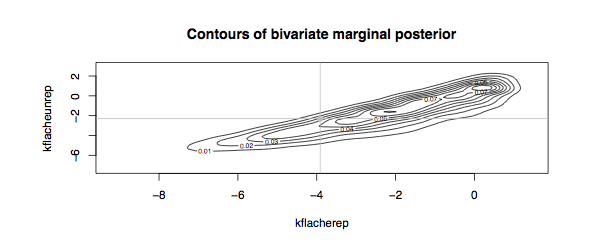
\includegraphics[height=2in,width=4in]{wilkinson_fig3_biv.png}
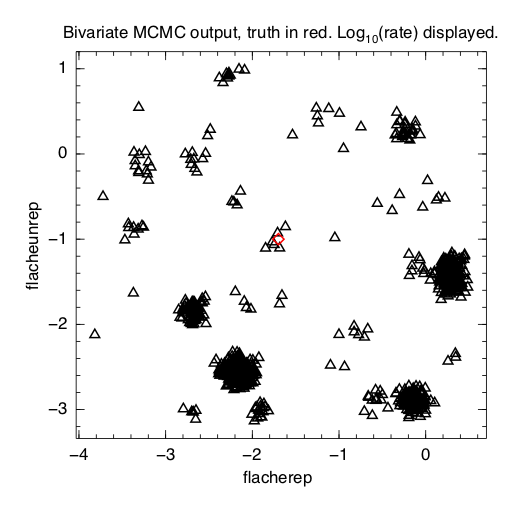
\includegraphics[height=4in,width=4in]{SigD_trial_may27.png}
\caption{Bivariate marginal of the posterior from Wilkinson's figure 3 (top) and my replication (bottom).}
\end{center}
\label{fig:SigD_trial_may27}
\end{figure}

%Some authors mention another method to maintain particle diversity: applying a different MCMC step whose kernel leaves the target invariant (see supplemental information of \cite{zechner2014scalable}). It is not clear that this applies

\subsubsection{Flexibility}
Wilkinson's approach is wonderfully adaptable. On the surface, Marjoram et al.'s LF-MCMC makes no HMM assumption and so is more flexible, but Wilkinson claims convincingly that LF-MCMC does not mix properly in this setting. The technique of constructing intermediate distributions by adding one datum at a time would generalize to any hidden Markov model, and coupled with the likelihood-free approach, this allows tremendous flexibility for indirect observation of stochastic and/or nonlinear systems. Adaptation for different types of observation (for example, a fluorescent protein instead of the protein of interest) is simple. Wilkinson points out that posteriors could be fed straight back into the algorithm as priors to analyze a second dataset, and this approach allows for analysis of different models that share parameters.

\subsubsection{Prior Selection}
In experiments, Wilkinson's priors cover four orders of magnitude, but they are centered (on a log scale) exactly over the true parameters. Are the results robust to choices of prior that merely cover the true values? \EMK{Experiment with that once you finish the replication.}

\subsection{Alternative Methods}
This area seems to have progressed rapidly starting around 2006: Reinker et al write in \cite{reinker2006parameter} that they are not aware of methods that can cope with measurement error in systems with few molecules. Now, in May of 2015, many strategies exist. Some, based on EM, are described in Section \ref{sec:intro_em}. Others include methods of moments, variational inference, and myriad adaptations of MCMC. My main concerns in assessing these models: predictive performance, tolerance for missing data, scaling, and uncertainty assessment.

Some schemes, such as \cite{milner2013moment}, \cite{kugler2012moment}, and \cite{zechner2012moment}, match moments to choose parameters. The core of these methods is an analytically-derived differential equation system that changes with the parameters. The system is typically infinite in size: only an infinite number of moments can completely encode the distributions that arise from the model. To facilitate a solution, higher moments are set to zero, and for each set of candidate parameters, the system is solved numerically. In \cite{milner2013moment}, the end result is a setup where quickly-solvable ODE's for mean and covariance give a Gaussian to approximate the true density, and \cite{milner2013moment} embeds this inside of a random-walk MCMC scheme. To distinguish this from LF-MCMC, it does evaluate an approximation to the likelihood: that is exactly what the moments are used for. MCMC also appears in \cite{zechner2012moment}, despite it falling in the ``method of moments'' category. The MCMC functions as a search algorithm to maximize an approximate posterior, which is evaluated as the prior times a moment-based normal approximation to the likelihood. Thus, these schemes require solving multidimensional ODE systems inside of MCMC samplers. The project  \cite{kugler2012moment} uses a penalty function involving higher moments, rather than a moment-matched approximate density. Despite being less interpretable in terms of statistics, the results in a fast procedure that allows for partial observations, as well as some assessment of uncertainty through repeated runs. For more information on different uses of moment closure, \cite{Milner201199} cites many applied projects using it. W09 precedes all of this work. 

Mean-field variational inference for Markov jump processes \cite{opper2008variational} scales well for large systems. This work precedes W09 by a year and has some intriguing properties. It is one of few inference methods in this subfield that requires no sampling or stochastic search, and it allows for fairly flexible priors on hidden states. W09's hidden state priors come implicitly from his parameter priors and initial state priors, meaning that in the hidden state, they treat only uncertainty due to intrinsic randomness, but in the parameters they treat uncertainty due to incomplete knowledge. Thus, (\cite{opper2008variational}) is a good option for inference when you want to fold in outside information about specific transitions.

To estimate parameters, \cite{opper2008variational} would need to be extended, perhaps as part of a variational EM algorithm. As written, the method produces only smoothed state estimates. Even variational EM does not give estimates of parameter uncertainty, so this work is not a viable alternative to W09 for scientific parameter estimation. For even more evidence that \cite{opper2008variational} cannot handle parameter estimation properly, the method performs well except for projection, and authors attribute this failure to untreated parameter uncertainty. 

James Rawlings' group has developed sampling algorithms that produce a semianalytical posterior distribution or likelihood over $\theta$, which they then optimize using derivative-free methods similar to simulated annealing \cite{gupta2014comparison,srivastava_rawlings2014stoch_opt}.   This work came after W09 by five years. They use an ingenious importance sampling scheme: if $q$ is the importance distribution, the idea starts as
\begin{align*}
P(\theta|D) &= \int_x P(\theta|x)P(x|D) dx\\
&\approx \sum_x P(\theta|x)\frac{P(x|D)}{q(x)} dx\\
&\approx \frac{1}{P(D)}\sum_x P(\theta|x)\frac{P(D|x)P(x)}{q(x)} dx.
\end{align*}
$P(D|x)$ is tractable. So is $P(\theta|x)$ if a conjugate gamma prior is used. They deal with $\frac{1}{P(D)}$ by normalizing the importance weights, and $P(x)$ they evaluate in closed form as $\frac{P(x|\theta)P(\theta)}{P(\theta|x)}$, which is a ratio of gamma distribution normalizing constants. This requires use of gamma priors, which is a restriction: the posterior is a mixture of many gammas, so it cannot be recycled as the prior of a new dataset. Also, domain experts 
often use log-normal or log-uniform priors, as does W09, and both sources regard prior choice as important. However, the scheme is exact, and well-designed $q$ can make it more efficient than MCMC-based schemes. If the prior choice issue could be resolved, this alternative might be well suited to Wilkinson's problem. 

As far as MCMC, a good place to start might be \cite{golightly2011bayesian}, because it seems to use every trick in the book. One numerical trick in particular bears mention: sometimes, likelihood terms appearing in proposal ratios can be replaced with noisy but unbiased estimates 
%
\footnote{Surprisingly, this works even with biased estimates, as long as the bias does not depend on the parameters being sampled.}
%
, and the target distribution will still be correct (details appear in \cite{andrieu2010particle}). This lets \cite{golightly2011bayesian} embed an SMC estimate of the intractable discrete-data likelihood inside of a random-walk MCMC scheme, retaining exactness. The price: noisier approximations at each step make for a slower mixing chain overall. Furthermore, the SMC inside the main loop requires forward simulations from the Gillespie algorithm. Displeased with the computational cost of SMC incurred at each iteration, \cite{golightly2011bayesian} employs another trick: they approximate the process using a continuous-state diffusion process satisfying a certain SDE. The SDE itself is intractable, so they use an Euler approximation to draw samples. Other papers using SDE approximations or related techniques include \cite{golightly2005bayesian} and
 \cite{fearnhead2014inference}.

Other non-exact methods include Approximate Bayesian Computation (ABC), which is compared with LF-MCMC in \cite{owen2014ABC_LF-MCMCcomparison}. 

Endpoint-conditioned simulation is the primary issue in this problem; it affects LF-MCMC, sampling-based EM schemes, and (indirectly, via the SMC estimate variance) the scheme in  \cite{golightly2011bayesian}. Thus, the paper \cite{amrein2012rate} is noteworthy for detailing a tidy, though approximate, solution. The set of eligible reaction totals given the change in chemical counts is phrased as a lattice; a matrix spanning it is obtained; it suffices to multiply a random vector of integers into that matrix. This work in \cite{amrein2012rate} is sophisticated enough to deal with partial measurements at a given time point, and it anticipates and deals with the criticism (e.g. \cite{golightly2011bayesian}) that separate block updates to parameters and latent state can lead to low acceptance rates.

Some MCMC methods are exact, with a general theme of using approximations to generate good proposals. For examples, \cite{owen2014scalable} uses a parallelized ABC algorithm and \cite{golightly2014smc_b_subtilis} explores several proposal-generating options, giving a particularly nice set of references in the process. %Some proposal schemes condition on the desired end-points of the bridge process \cite{hobolth2009simulation}, but \cite{hobolth2009simulation} assumes a finite state space. 
The paper \cite{zechner2014scalable} is similar to Wilkinson's, using MCMC updates inside a sequential Monte Carlo scheme. They use a more complex model that treats batches of cells with some shared parameters and some parameters that vary by cell. The mathematical machinery involves extra tools to marginalize over between-cell variability and block updates in places where Wilkinson doesn't need them.

%\begin{figure}[h!]
%\begin{center}
%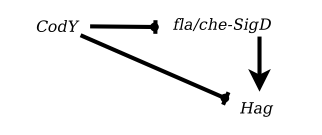
\includegraphics[scale=0.5]{wilkinson_reg_network.png}
%\caption{Regulatory relationships. $Hag$ is the gene for $flagellin$, while $SigD$ encodes $\sigma^D$.}
%\end{center}
%\label{fig:}
%\end{figure}


\begin{align*}
\end{align*}
\begin{align*}
\end{align*}
\begin{align*}
\end{align*}
\begin{align*}
\end{align*}

%\texttt{code snippet}
%
%\begin{algorithm}[h]
%\caption{ }
%Do things\\
%Loop:\\
%\Indp
% Do this again and again\\
%\end{algorithm}

%\begin{figure}[h!]
%\begin{center}
%\includegraphics[height=4in,width=6in]{filename.pdf}
%\caption{}
%\end{center}
%\label{fig:}
%\end{figure}

%$\left[
%\begin{tabular}{ >{$}c<{$} >{$}c<{$}}
% 1 & -\phi_1\\
% -\phi_1 & 1
%\end{tabular} 
%\right]$

%==== Bib files and style =======
\bibliographystyle{splncs}
\bibliography{prelim_biblio}
\end{document}
